
\documentclass[aspectratio=169,11pt]{beamer}
% customize block aesthetics
\definecolor{customblue}{rgb}{0.13,0.28,0.59}
\setbeamercolor{block title}{bg=customblue, fg=white}
\setbeamercolor{block body}{bg=customblue!10}
\setbeamertemplate{blocks}[rounded]
\usepackage{array,color,graphicx,comment,tikz}
\usepackage{bibentry}
\bibliographystyle{abbrv}
\setbeamertemplate{bibliography entry title}{}
\setbeamertemplate{bibliography entry location}{}
\setbeamertemplate{bibliography entry note}{}
\setbeamercolor{bibliography entry author}{fg=black}
\setbeamercolor{bibliography entry title}{fg=gray}
%\usetikzlibrary{calc,patterns,decorations.pathmorphing,decorations.markings}
\input talk_defs.tex
%\input formatting.tex

\mode<presentation>
{
\usetheme{default}
}

\setbeamertemplate{navigation symbols}{}
\usecolortheme[rgb={0.13,0.28,0.59}]{structure}
\setbeamertemplate{itemize subitem}{--}
\newcommand\footlineon{
\setbeamertemplate{footline} {
\begin{beamercolorbox}[ht=2.5ex,dp=1.125ex,leftskip=.8cm,rightskip=.6cm]{structure}
%\footnotesize \insertsection
\hfill
{\insertframenumber}
\end{beamercolorbox}
\vskip 0.45cm
}
}
\footlineon

\AtBeginSection[] 
{ 
	\begin{frame}<beamer> 
		\frametitle{Outline} 
		\tableofcontents[currentsection,currentsubsection] 
	\end{frame} 
} 

%% begin presentation
\title{
REGROW: Renewable Energy Generation Risk from Outlier Weather
}

\author{\textbf{Giray Ogut} \and Bennet Meyers \and Stephen Boyd\\
}
\institute{\normalsize Stanford University}

\date{\small Cybersecurity and Technology Innovation Conference, 7/31/2024}

\begin{document}

\begin{frame}
\titlepage
\end{frame}

\begin{frame}{Overview}
\BIT
\item \textbf{objective:} Model power generation of a PV system with seasonal variation
\item \textbf{application:} Estimate marginal quantiles and detect for clear sky intervals
\item \textbf{approach:} White-box ML model using convex optimization \\
\hspace{12mm} $-$ low computational requirements (\eg \ single laptop) \\
\hspace{12mm} $-$ works with missing data (even after removing \% 70) \\
\hspace{12mm} $-$ interpretable and auditable results
\vspace{5mm}
\item \textbf{prior work:} Physical models using geographic coordinates, atmospheric parameters etc.
\small{[Kambezidis1997,Stein2012, Antonanzas2019]} or
black-box models such as neural networks \small{[Zhandire2017,Mosaico2019, Masucco2019]}  
\EIT
\end{frame}

\begin{frame}{Bundt cake representation}
\BIT
\item express daytime, time dilated data $X \in (\reals_+ \cup \{?\})^{D \times M}$
as a ''Bundt" cake
\item $D$ is the number of days and $M$ is the number of intervals in a day
\item allow for missing data $X_{d,m} = \ ?$
\EIT
\vspace{-8mm}
	\begin{columns}
		\begin{column}{0.5\textwidth}
			\begin{figure}
				\centering
				\includegraphics[width=\columnwidth]{../figs/cake.pdf}
			\end{figure}
		\end{column}
		\begin{column}{0.5\textwidth}
			\begin{figure}
				\centering
				\includegraphics[width=\columnwidth]{../figs/toast.pdf}
			\end{figure}
		\end{column}
		\end{columns}
\end{frame}

\begin{frame}{Bundt cake representation (continued)}
\BIT
\item each ''slice" of the cake corresponds to a day
\item slices start and end near zero (\ie \ standing waves)
\item allows comparison of different days on equal footing
\begin{figure}
\centerline{\includegraphics[width=\columnwidth,keepaspectratio,clip=true]{../figs/slices.pdf}}
\end{figure}
\EIT
\end{frame}

\begin{frame}{Method}
\BIT
\item to get from raw data to Bundt cake representation, we do \\

$-$ PV sunrise/sunset estimation \\
$-$ time dilation

\vspace{5mm}
\item using Bundt cake representation, we can \\
$-$ estimate marginal quantiles \\
$-$ detect clear sky
\EIT
\end{frame}

\begin{frame}{Fitting smooth multiperiodic basis functions}
\BIT
\item define a set of basis functions, 
$\phi_i \quad i=1,\ldots,N$ such as 
\[
\cos (2\pi 3t/P_1), \qquad 
\sin (\pi t/P_2), \quad
\cos (2\pi 3 t/P_1) \sin (\pi t/P_2)
\]
\item more sophisticated bases such as splines can also be used
\item express any model parameter $\theta \in \reals$ as
\[
	\theta = \sum_{i=1}^N \alpha_i \phi_i(t).
\]
\item fitting the coefficients $\alpha_i$ is formulated 
as a convex optimization problem 

\item see our paper \& open source package 
\url{https://stanford.edu/~boyd/papers/bundt.html}
\&
\texttt{pip install spcqe}
\EIT
\end{frame}

%\section{Example}

\begin{frame}{Numerical example}
\begin{columns}
	\begin{column}{0.5\textwidth}
		\begin{figure}
			\centering
			\includegraphics[width=\columnwidth]{../figs/fig2.pdf}
		\end{figure}
	\end{column}
	\begin{column}{0.5\textwidth}
		\BIT
		\item residential PV system in Southern California
		\item 15-minute average power from 07/01/2015 to 06/30/2016
		(no missing data)
		\item clear seasonal and
		daily patterns
		\item shade in winter, fog early in the day during summer
		\EIT
	\end{column}
\end{columns}
\end{frame}

\begin{frame}{Smooth PV sunrise/sunset estimation}
\BIT
\item PV sunrise/sunset is different from astronomical sunrise/sunset
\item basic thresholding results in noisy estimates and multiple transitions in a day
\item we come up with smooth estimates
\EIT
	\begin{columns}
		\begin{column}{0.5\textwidth}
			\begin{figure}
				\centering
				\includegraphics[width=\columnwidth]{../figs/basic_sunrise_sunset.pdf}
			\end{figure}
		\end{column}
		\begin{column}{0.5\textwidth}
			\begin{figure}
				\centering
				\includegraphics[width=\columnwidth]{../figs/fig3.pdf}
			\end{figure}
		\end{column}
	\end{columns}

\end{frame}

\begin{frame}{Time dilation}
\BIT
\item identify daytime between estimated sunrise and sunset
\item map each daytime interval to a fixed period $M$
\item time dilation preserves the energy of the signal (\ie \ same area under the curve)
\EIT
\begin{figure}
\centerline{\includegraphics[width=\columnwidth,keepaspectratio,clip=true]{../figs/time_dilate.pdf}}
\end{figure}
\end{frame}

\begin{frame}{Time dilation (continued)}
\begin{columns}
	\begin{column}{0.5\textwidth}
		\begin{figure}
			\centering
			\includegraphics[width=\columnwidth]{../figs/time_dilation.pdf}
		\end{figure}
	\end{column}
	\begin{column}{0.5\textwidth}
		\BIT
			\item shorter days are dilated more
			\item we can compare different days on equal footing 
		\EIT
	\end{column}
\end{columns}

\end{frame}




\begin{frame}{Smooth marginal quantiles}
\begin{columns}
	\begin{column}{0.5\textwidth}
		\begin{figure}
			\centering
			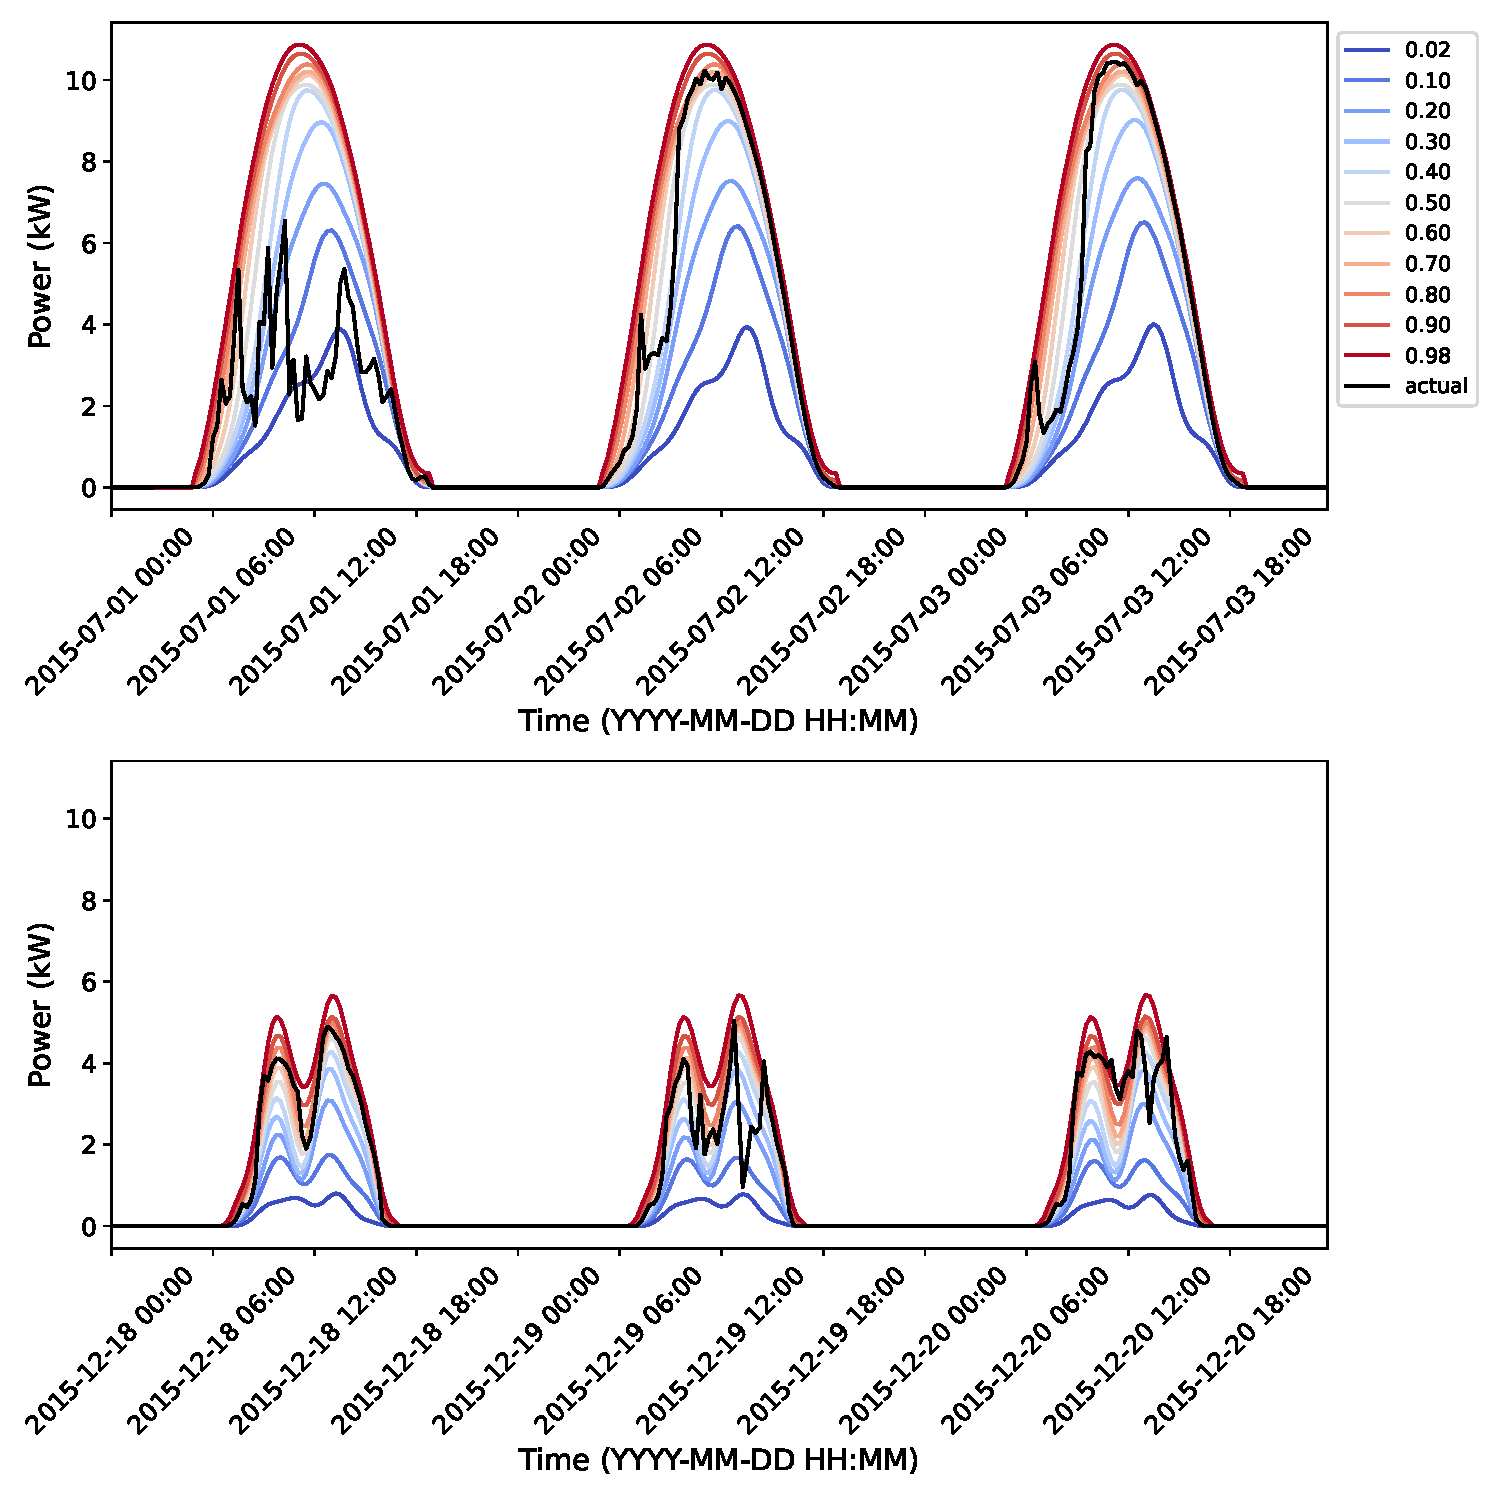
\includegraphics[width=\columnwidth]{../figs/quantiles_mapped_back.pdf}
		\end{figure}
	\end{column}
	\begin{column}{0.5\textwidth}
		\BIT
		\item estimating quantiles means estimating CDF at each time
		\item very powerful: estimate whole distribution from a single point!
		\item quantiles adapt to the seasonal variation
		\item quantiles can be used for various applications
		such as anomaly detection, missing data infill, etc.
		\EIT
	\end{column}
\end{columns}
\end{frame}

\begin{frame}{Clear sky detection}

\BIT
\item na\"{i}ve method: thresholding on clear sky index
\item leads to many transitions between clear and 
non clear sky intervals
\item introduce a post-processing step that smooths 
out clear sky estimate  
\EIT

\begin{columns}
	\begin{column}{0.5\textwidth}
		\begin{figure}
			\centering
			\includegraphics[width=0.9\columnwidth]{../figs/naive_clear_sky.pdf}
		\end{figure}
	\end{column}
	\begin{column}{0.5\textwidth}
		\begin{figure}
			\centering
			\includegraphics[width=0.9\columnwidth]{../figs/clear_sky.pdf}
		\end{figure}
	\end{column}
\end{columns}


\end{frame}

\begin{frame}{Clear sky detection (continued)}
\BIT 
\item form graph: 2 nodes/interval (clear, non-clear)
\item detected clear sky is the shortest 
path which minimizes transitions and mismatches
\item solve for each day separately using dynamic programming ($\mathcal{O}(M)$)
\EIT

\begin{figure}
\centerline{\includegraphics[width=\columnwidth,keepaspectratio,clip=true]{../figs/clear_sky_graph.pdf}}
\end{figure}
\end{frame}




\begin{frame}{Conclusion \& next steps}
	\BIT
	\item introduced a white-box ML model for power output of a \emph{single} PV system
	\item showed how to estimate quantiles and detect clear sky intervals 
	\vspace{5mm}
	\item will start fleet scale analysis with \emph{multiple} PV systems
	\item do joint Gaussianization and copulas
	\item include heterogeneous data (temperature, wind, etc.) in analysis
	\EIT
	\vspace{5mm}
	{\footnotesize This material is based on work supported by the U.S. Department of Energy's Office of
	Energy Efficiency and Renewable Energy (EERE) under the Solar Energy Technologies Office
	Award Number 38529.}
\end{frame}
	

\end{document}
